\documentclass[varwidth=true, border=2pt]{standalone}
\usepackage{tikz}
\usetikzlibrary{arrows,positioning}
\tikzset{
    %Define standard arrow tip
    >=stealth',
    % Define arrow style
    pil/.style={->,thick}
}

\begin{document}
  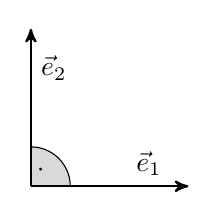
\begin{tikzpicture}
    \draw[fill=gray!30, label=$a$] (0,0) -- node[above, near start] {$\cdot$} (0.5,0)
                        arc (0:90:0.5cm);
    \draw[pil] (0,0) -- node[near end, above] {$\vec e_1$} (2cm, 0);
    \draw[pil]  (0,0) -- node[near end, right] {$\vec e_2$} (0, 2cm);
  \end{tikzpicture}
\end{document}
